\section{计算机视觉基础模型}

深度学习技术不仅推动着自然语言处理技术的发展与革命,其在早期更是在计算机视觉领域推动者各项技术从研究起步迈向成熟落地。相比于自然语言处理技术在近年来才迎来应用热潮,计算机视觉中的相关研究则早已应用到生产生活中。这也是目前大部分融合视觉信息的自然语言处理任务均应用预训练好的计算机视觉基础模型对图像进行编码的原因。

融合图片信息的神经机器翻译任务需要将图片信息输入到神经机器翻译模型中,因此同样需要采用神经网络方法对图片信息编码。针对不同的翻译模型选择合适的图片编码方法,能够提升视觉信息在翻译模型中的作用,从而帮助提升翻译模型的性能。目前ImgNMT中融合图片信息的方式主要可以分为三类:图片全局信息、图片动态局部信息以及视觉目标信息。本节,我们将主要针对这三类图片信息作用方式介绍其背后的计算机视觉基础模型。

% 基础模型在ImgNMT中的利用:
%   CNN:全局特征、栅格特征
%   R-CNN:视觉目标特征
%   visual grounding:(短语,视觉目标特征)

\subsection{卷积神经网络}

卷积神经网络是目前计算机视觉领域最重要且最流行的方法之一,可以在计算机视觉的多个研究任务中发挥重要作用,例如图像分类、目标检测、人脸识别、语义分割等。早在20世纪90年代,杨·乐坤(Yann LeCun)等人发表论文提出了LeNet-5,成为奠定了现代卷积神经网络方法的基础框架\cite{fukushima1980neocognitron,DBLP:journals/pieee/LeCunBBH98,lecun1989handwritten}。
现有的卷积神经网络,如AlexNet\cite{DBLP:conf/nips/KrizhevskySH12},VGGNet\cite{DBLP:journals/corr/SimonyanZ14a},GoogLeNet\cite{DBLP:journals/corr/SzegedyLJSRAEVR14},ResNet\cite{32_DBLP:conf/cvpr/HeZRS16},DenseNet\cite{DBLP:conf/cvpr/HuangLMW17}等模型,均是在LeNet-5的基础上通过加深网络层数、增加或改变非线性激活层、增加批数据归一化、增加通道数量等手段提升网络的泛化性能和对图像的表征能力。卷积神经网络不仅在计算机视觉领域得到广泛应用,在语音识别和自然语言处理的某些特定任务上同样得到了关注。在融合图像信息的多模态任务上,卷积神经网络更是用于表征图片信息或视频信息的必然选择。本节将以LeNet-5为例,详细介绍卷积神经网络的基本结构,以及应用到跨模态信息融合时的使用方式。

\begin{figure}[!htbp]
    \centering
    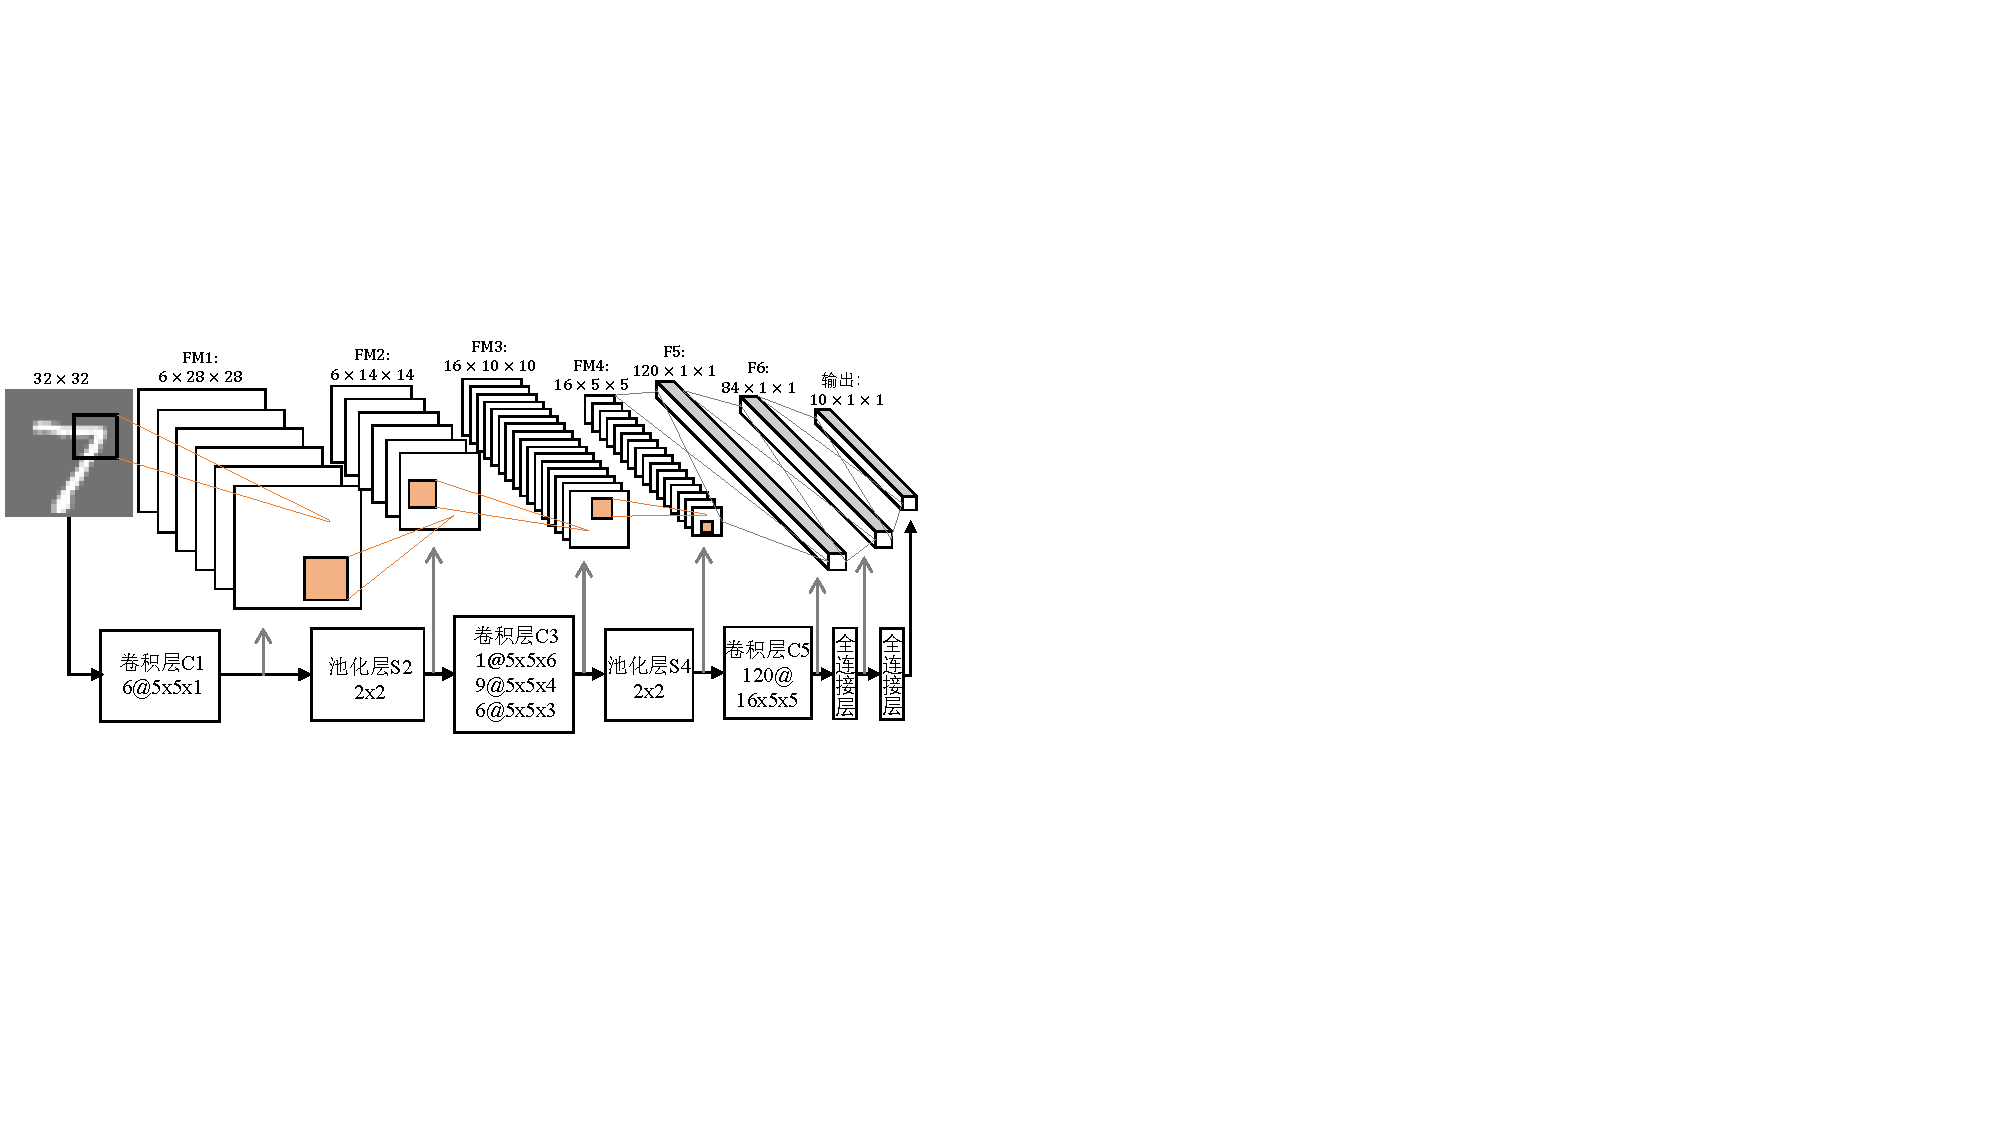
\includegraphics[scale=0.9]{Img/fig_2_lenet5.pdf}
    \bicaption{LeNet-5模型示意图}{Schematic diagram of the LeNet-5 model}
    \label{fig:2_lenet5}
\end{figure}
LeNet-5是最早的卷积神经网络模型之一,设计之初被用于手写数字识别任务。图\ref{fig:2_lenet5}展示了LeNet-5从输入图片到输出预测结果的模型工作简化图。LeNet-5共包含5层,包括两个卷积层(convolutional layer)C1、C3、C5,以及两个池化层(pooling layer)S2和S4。

{\sffamily 卷积层:}卷积层是CNN模型的核心模块,包含了整个模型的大部分参数。它可以对输入图像的局部区域进行加权求和从而得到图片的特征(feature)或特征图(feature map,FM),例如示例中经过卷积层得到的特征或特征图有FM1、FM3和F5。卷积层中卷积核(convolution kernel)大小和形状的选择能够影响卷积的效果。例如,图\ref{fig:2_lenet5}中卷积层C1中有6个$5 \times 5 \times 1$的卷积核,每个卷积核将图片中每个$5 \times 5$大小区域内的像素点加权求和得到输出特征图中的一个像素点,那么一个$32 \times 32$大小的图片经过卷积层C1后得到的特征图FM1的大小为$6 \times 28 \times 28$。经过卷积层后,图片的通道数可能会增加,图片的尺寸也可能变小。卷积层的设计可以很简单也可以非常的复杂,例如卷积层C3中包含了16个卷积核,其中各卷积核的尺寸为$5 \times 5$,但选取的特征图数量(图中包含6,4,3三种数量的差别)却各不相同。这说明卷积层的设计可以是非常灵活的,也因此对模型设计与研究人员的考验也是巨大的。

{\sffamily 池化层:}池化层一般也成为下采样层(subsampling layer),相当于一个过滤器,对图片或特征图执行降维操作,滤掉无用的像素点,帮助模型提取更高层次的特征。其原理是在输入特征图中一个局部区域内,按照选取最大值或计算平均值的方式为输出特征图增加一个新的像素点,也称最大池化(max pooling)和平均池化(average pooling)。例如图\ref{fig:2_lenet5}中的池化层S2的大小为$2 \times 2$,它在图片中对应区域内选取最大值或计算平均值后输出到特征图FM2中。区别于卷积层,池化层对输入特征图进行过滤像素时,一般不设置重叠区域,例如图中的池化层的尺寸和步长均为2,因此特征图经过池化层后特征图的尺寸变为原来的二分之一。

{\sffamily 全连接层:}全连接层(full connection layer)层中的每个神经元都连接着上一层的所有神经元。区别于卷积层和池化层将图片映射到隐层的特征空间中,而全连接层将隐层表示映射为图片的分布式特征表示,或经过非线性激活函数(一般采用softmax函数)得到样本的概率模型并预测样本的分类结果。例如图\ref{fig:2_lenet5}中最后的全连接层将图片特征F6映射为一个维度为10的向量中,每个维度的取值为0到1,代表着预测为0到9每个值的概率。

虽然LeNet-5的结构简单,但依旧展现了卷积神经网络能够学习并表征图片信息的能力。层数更深,网络结构更复杂,以及采用了更多新技术的新一代卷积神经网络能够表征更复杂的图像信息。在融合视觉信息的自然语言处理任务中,因文本输入与图片输入很难在一个模型中同时支持,因此通常采用特征融合的方式支持多模态输入。从一般的卷积神经网络的模型结构可以看到,选取图片特征的选择可以有很多种。例如图\ref{fig:2_lenet5}中FM4的尺寸为$16 \times 5 \times 5$,其中,在$5 \times 5$的特征图内仍保留着与源图片中的区域对应关系。因此FM4可看作是由$5 \times 5$个维度为16的特征组合而成,每个16维的特征表征了图片中对应的区域。这种保留了图片内局部空间信息的特征图一般称为栅格特征(grid feature)或局部特征(local feature)。在融合图片信息的神经机器翻译方法中,栅格特征一般可以作为图片输入序列输入到翻译模型中,通过注意力机制能够动态地关注到栅格特征中保留的局部空间信息。利用平均池化将栅格特征所代表的多个视觉特征融合为一个视觉特征,称作全局特征(global feature)。全局特征表征了图片的完整信息,通常可以用于初始化循环神经网络,或作为词向量等方式输入到神经机器翻译模型中。

% 要强调栅格信息保留了位置信息
% 这里最好直接举ResNet的例子,可以直接将残差连接的引入到现有机器翻译模型中

\subsection{目标检测方法}

% R-CNN:two-stage
%      R-CNN-> Fast R-CNN -> Faster R-CNN
% Yolo v0-5: one-stage
%      v0: 遍历所有“框” -》 输出(c,x,y,w,h) 其中c为confidence,label为(1,x*,y*,w*,h*)
%      v1:检测多个目标,将img划分为多个区域,(c,x,y,w,h,one-hot)*N
% visual grounding

\subsection{视觉Transformer}
%这里和前面呼应以下,前面是CV推动着NLP的发展,这里则反过来,NLP推动CV

% 结尾说以下那几篇文章说过使用哪种CNN-backbone带来的差别并不大